%%%%%%%%%%%%%%%%%%%%%%%%%%%%%%%%%%%%%%%%%%%%%%%%%%%%%
%
%  Template
%  Beamer Presentation by Chris Bourke
%
%%%%%%%%%%%%%%%%%%%%%%%%%%%%%%%%%%%%%%%%%%%%%%%%%%%%%%%%%%%%%%%%%%%%%%%

\documentclass[]{beamer}
%\documentclass[handout]{beamer}

\geometry{papersize={16cm,9cm}}

% For handout version:
%\usetheme[hideothersubsections,slidenumbers]{UNLTheme}
\usetheme[hideothersubsections]{UNLTheme}
\usepackage{amssymb}
\input{StandardCommands}
\usepackage[linesnumbered,ruled,vlined]{algorithm2e}
\SetKwComment{Comment}{//}{}
\DontPrintSemicolon
\SetKwSty{textsc} %
%\SetAlFnt{\scriptsize} %
\SetKwInOut{Input}{Input} %
\SetKwInOut{Output}{Output} %
%\setalcapskip{1em} % changed to
\SetAlCapSkip{1em}
\setlength{\algomargin}{2em} %
%\Setvlineskip{0em} % changed to:
\SetVlineSkip{0em}

\usepackage{tikz}
\usetikzlibrary{fadings}
\usetikzlibrary{shapes.geometric,shapes.symbols}
\usetikzlibrary{calc,shapes.multipart,chains,arrows}
\usetikzlibrary{arrows.meta,calc,shapes.multipart,chains,arrows}
%\usetikzlibrary{calc,shapes.multipart,chains,arrows}
%%\usetikzlibrary{backgrounds}
\usetikzlibrary{backgrounds}
\usetikzlibrary{decorations.pathreplacing}
\usetikzlibrary{decorations.pathmorphing}
\tikzset{onslide/.code args={<#1>#2}{%
  \only<#1>{\pgfkeysalso{#2}} % \pgfkeysalso doesn't change the path
}}
\tikzset{temporal/.code args={<#1>#2#3#4}{%
  \temporal<#1>{\pgfkeysalso{#2}}{\pgfkeysalso{#3}}{\pgfkeysalso{#4}} % \pgfkeysalso doesn't change the path
}}

\tikzset{
    fading speed/.code={
        \pgfmathtruncatemacro\tikz@startshading{50-(100-#1)*0.25}
        \pgfmathtruncatemacro\tikz@endshading{50+(100-#1)*0.25}
        \pgfdeclareverticalshading[%
            tikz@axis@top,tikz@axis@middle,tikz@axis@bottom%
        ]{axis#1}{100bp}{%
            color(0bp)=(tikz@axis@bottom);
            color(\tikz@startshading)=(tikz@axis@bottom);
            color(50bp)=(tikz@axis@middle);
            color(\tikz@endshading)=(tikz@axis@top);
            color(100bp)=(tikz@axis@top)
        }
        \tikzset{shading=axis#1}
    }
}

\usepackage{multirow}
\usepackage{multicol}

\definecolor{steelblue}{rgb}{0.2745,0.5098,0.7059}
\hypersetup{
    colorlinks = true,
    urlcolor = {steelblue},
    linkbordercolor = {white}
}

\definecolor{mintedBackground}{rgb}{0.95,0.95,0.95}
\definecolor{mintedInlineBackground}{rgb}{.90,.90,1}

%\usepackage{newfloat}
\usepackage{minted}
\setminted{mathescape,
               linenos,
               autogobble,
               frame=none,
               fontsize=\small,
               framesep=2mm,
               framerule=0.4pt,
               %label=foo,
               xleftmargin=2em,
               xrightmargin=0em,
               startinline=true,  %PHP only, allow it to omit the PHP Tags *** with this option, variables using dollar sign in comments are treated as latex math
               numbersep=10pt, %gap between line numbers and start of line
               style=default, %syntax highlighting style, default is "default"
               			    %gallery: http://help.farbox.com/pygments.html
			    	    %list available: pygmentize -L styles
               bgcolor=mintedBackground} %prevents breaking across pages
               
\setmintedinline{bgcolor={mintedInlineBackground}}
\setminted[text]{bgcolor={},linenos=false,autogobble,xleftmargin=1em}


\title[~]{Computer Science I}
\subtitle{Basics}
\author[~]{Dr.\ Chris Bourke\\ \email{cbourke@cse.unl.edu}} %
\date{~}



\begin{document}

\begin{frame}
  \titlepage
\end{frame}

\setbeamertemplate{section in toc}{\inserttocsectionnumber.~\inserttocsection}
\setbeamercolor{section in toc}{fg=black}
%\setbeamertemplate{subsection in toc}{~} %\inserttocsubsection\\}

\begin{frame}
  \frametitle{Outline}
%{\footnotesize
%\begin{NoHyper}
%  \tableofcontents[hideallsubsections]
%\end{NoHyper}
%}

\setbeamercolor{enumerate item}{bg=white,fg=black}
\setbeamercolor{item}{bg=white,fg=black}
\setbeamercolor{item projected}{bg=white,fg=black}
\setbeamercolor{enumerate subitem}{fg=red!80!black}
\setbeamertemplate{enumerate items}[default]
\begin{enumerate}
  \item Introduction
  \item Variables \& Operators
  \item Basic I/O
  \item Exercises
  %\item Coding Style
  \item Noninteractive Input
  \item Toolkit: Linters
\end{enumerate}

\end{frame}

\section{Introduction}

\begin{frame}
    \frametitle{}
    \framesubtitle{}
    
    \begin{center}
    {\Huge Part I: Introduction}\\
    {\Large Overview, Compiling, Elements of a Program}
    \end{center}

\end{frame}

\begin{frame}
    \frametitle{Overview}
    \framesubtitle{}

\begin{itemize}[<+->]
  \item A \emph{computer program} is a collection of instructions
that performs a specific task when executed by a computer

  \item A \emph{programming language} is a formal language that 
specifies a set of instructions that can be used in a program

  \item We write programs in a code (text) editor or Integrated
  Development Environment (IDE)
  
  \item Source code is is \emph{compiled} and run on a particular
  \emph{operating system}
\end{itemize}

\end{frame}

\begin{frame}
    \frametitle{Process}
    \framesubtitle{}  
    
\begin{itemize}[<+->]
  \item \emph{Source code} -- plain text files containing computer code.

  \item \emph{Assembly} -- a low-level programming language
  closer to a processor's actual ``language''
  
  \item \emph{Machine Code} -- set of instructions executed directly 
  by a computer's central processing unit (CPU)

  \item \emph{Binary} -- a sequence of 0s and 1s 
\end{itemize}

\onslide<5>{
$$\textrm{source} \rightarrow \textrm{assembly} \rightarrow \textrm{machine}$$
}

\end{frame}

\begin{frame}
    \frametitle{Compiling}
    \framesubtitle{}

\begin{center}
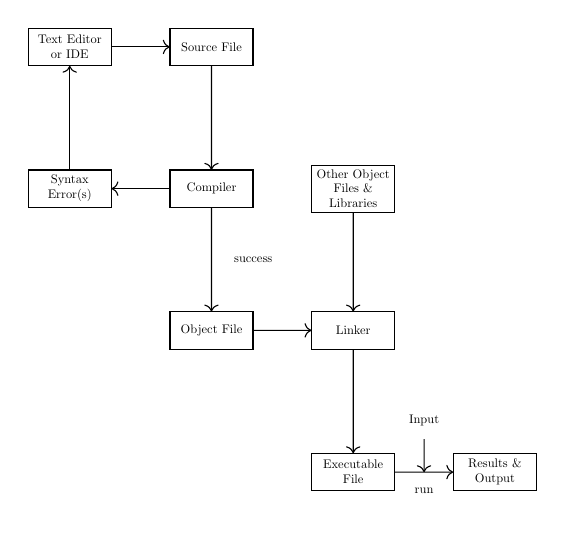
\begin{tikzpicture}[auto,scale=0.45,transform shape,every node/.style={draw,text width=6em,node distance=4cm,text badly centered,minimum height=3em}]

% Define block styles
\tikzstyle{decision} = [diamond, draw, fill=yellow!20,
    text width=4.5em, text badly centered, node distance=5cm, inner sep=0pt]
\tikzstyle{block} = [rectangle, draw, fill=green!20,
    text width=5em, text centered, rounded corners, minimum height=4em, node distance=5cm]
\tikzstyle{line} = [draw, -latex']; %
\tikzstyle{cloud} = [rectangle,rounded corners,draw,fill=blue!20, node
distance=5cm, minimum height=2em, text width=5em];

\node [] (ide) {Text Editor or IDE};
\node [right of=ide] (source) {Source File};
\node [below of=source] (compiler) {Compiler};
\node [below of=ide] (error) {Syntax Error(s)};

\node [below of=compiler] (object) {Object File};
\node [right of=object] (linker) {Linker};
\node [above of=linker] (libraries) {Other Object Files \& Libraries};

\node [below of=linker] (executable) {Executable File};

\node [right of=executable] (results) {Results \& Output};

\draw[->] (ide.east) -- (source.west);
\draw[->] (source.south) -- (compiler);

\draw[->] (compiler) -- (error);

%\draw[->] (compiler.west) -- node[pos=.50,draw=none,below,text width=5em] {syntax error(s)} (error.east);

\draw[->] (error) --  (ide);
\draw[->] (compiler) -- node[pos=.50,draw=none] {success}  (object);
\draw[->] (object) --  (linker);
\draw[->] (libraries) --  (linker);
\draw[->] (linker) --  (executable);

\draw[->] (executable) -- node[pos=.50,draw=none,below,text width=5em] (run) {run} (results);

\node [above of=run,draw=none,node distance=2cm] (input) {Input};

\draw[->] (input) -- (run);

\end{tikzpicture}
\end{center}

\end{frame}

\begin{frame}
    \frametitle{Demonstration}
    \framesubtitle{}

\begin{itemize}
  \item Edit a source file, \mintinline{text}{hello.c}
  \item Assemble: \\
  \mintinline{text}{gcc -S hello.c}
  \item Compile: \\
  \mintinline{text}{gcc -c hello.c}
  \item View binary/hex: \\
  \mintinline{text}{hexdump -C hello.o}
  \item All in one:
  \mintinline{text}{gcc hello.c}
  \item Run:
  \mintinline{text}{./a.out}
\end{itemize}

\end{frame}


\begin{frame}[fragile]
    \frametitle{Example}
    \framesubtitle{}

\begin{minted}[fontsize=\tiny]{c}
/**
 * Author: Chris Bourke
 * Date: November 2, 2016
 *
 * This program converts miles to kilometers
 */
#include<stdlib.h>
#include<stdio.h>

#define KMS_PER_MILE 1.60934

int main(int argc, char **argv) {

  double miles, kms;

  printf("Please enter miles: ");

  scanf("%lf", &miles);

  kms = KMS_PER_MILE * miles;

  printf("%f miles is equal to %f kilometers\n", miles, kms);

  return 0;
}
\end{minted}

\end{frame}

\begin{frame}[fragile]
    \frametitle{Comments \& Documentation}
    \framesubtitle{}

\begin{itemize}[<+->]
  \item Comments are human-readable messages embedded in code
  \item Single line comments: \mintinline{c}{// this is a comment}
  \item Multiple line comments: 
\begin{minted}{c}
/* This is a multiline 
   comment. */
\end{minted}
\end{itemize}

\end{frame}

\begin{frame}[fragile]
    \frametitle{Comments \& Documentation}
    \framesubtitle{}

\begin{itemize}[<+->]
  \item ``Doc-style'' comments:
\begin{minted}{c}
/**
 * This is a doc-style comment.  It is
 * a multiline comment commonly used for
 * large blocks of documentation comments
 */
\end{minted}
  \item Comments should tell you the \emph{what} and the \emph{why}
  \item Code should be self-documenting, code itself should tell the \emph{how}  
\end{itemize}

\end{frame}

\begin{frame}[fragile]
    \frametitle{Preprocessor Directives}
    \framesubtitle{}

\begin{itemize}[<+->]
  \item Preprocessor directives tell the compiler to do 
  certain things to the source code before compiling
  \item Begin with a hash \mintinline{c}{#}
  \item Macros: \mintinline{c}{#define a b} 
  \item Macro usage: defining constants; avoiding ``magic'' numbers
  \item Including libraries: 
\begin{minted}{c}
#include<stdlib.h>
#include<stdio.h> 
#include<math.h> 
\end{minted}
\end{itemize}  
    
\end{frame}

\begin{frame}[fragile]
    \frametitle{Main Function}
    \framesubtitle{}

\begin{itemize}[<+->]
  \item The \mintinline{c}{main} function is the main entry point 
  of a program
  \item Without a \mintinline{c}{main} a program is not \emph{executable}
  \item Input/output functions: \mintinline{c}{scanf}, \mintinline{c}{printf}
  \item Math functions: \mintinline{c}{sqrt}, \mintinline{c}{sin}, \mintinline{c}{pow}
\end{itemize}

\end{frame}

\begin{frame}[fragile]
    \frametitle{Syntax \& Punctuation}
    \framesubtitle{}

\begin{itemize}[<+->]
  \item In general, executable lines ends with a semicolon \mintinline{c}{;}
  \item \emph{Blocks} of code are delimited by opening and closing curly brackets \mintinline{c}{{ ... }}
  \item Commas \mintinline{c}{,} are used to delimit arguments, variables, etc.
  \item In general, whitespace does not affect a program
  \item Keywords: \mintinline{c}{int}, \mintinline{c}{double}, \mintinline{c}{return}
\end{itemize}
  
\end{frame}


\section{Variables \& Operators}

\begin{frame}
    \frametitle{}
    \framesubtitle{}
    
    \begin{center}
    {\Huge Part II: Variables \& Operators}\\
    {\Large ~}
    \end{center}

\end{frame}

\begin{frame}[fragile]
    \frametitle{Variables}
    \framesubtitle{}

\begin{itemize}[<+->]
  \item Variables are program elements that hold \emph{values} that can be \emph{assigned} and \emph{reassigned}
  \item C is a \emph{statically typed} language
  \item All variables have a name (\emph{identifier}) and a fixed \emph{type}
  \item Types: integers, floating-point (decimal) numbers, characters, etc.
  \item Variables must be \emph{declared} before they can be used
  \item The \emph{scope} of a variable is the section(s) of code in which it exists
\end{itemize}

\end{frame}

\begin{frame}[fragile]
    \frametitle{Basic Types}
    \framesubtitle{Integers}

\begin{itemize}[<+->]
  \item An integer variable: \mintinline{c}{int}
  \item A 32-bit signed two's complement integer variable
  \item Can represent values:
    $$-2^{31} = -2,147,483,648 \leq x \leq 2,147,483,647 = 2^{31} - 1$$
  \item Examples:
\begin{minted}{c}
int x;
int numberOfStudents = 42;
int golfScore = -3;
\end{minted}
\end{itemize}

\end{frame}

\begin{frame}[fragile]
    \frametitle{Basic Types}
    \framesubtitle{Floating Point Numbers}

\begin{itemize}[<+->]
  \item A \mintinline{c}{double} is a decimal number
  \item A 64-bit ``floating'' point number
  \item Similar to scientific notation:
  $$3895.434 \rightarrow 3.895434 \times 10^{3}$$
  $$-0.0043 \rightarrow -4.3 \times 10^{-3}$$
  \item Decimal values accurate to 16--17 digits %emphasize limitations 
  \item Another: \mintinline{c}{float} (avoid, less precise)
  \item Examples:
\begin{minted}{c}
double pi = 3.14159;
double totalCost = 3219.32;
\end{minted}
\end{itemize}

\end{frame}

\begin{frame}[fragile]
    \frametitle{Basic Types}
    \framesubtitle{Single Characters}

\begin{itemize}[<+->]
  \item A \mintinline{c}{char} is a single character
  \item American Standard Code for Information Interchange (ASCII) character %1960
  \item Examples:
\begin{minted}{c}
char firstInitial = 'C';
char response = 'y';
\end{minted}
\end{itemize}

\end{frame}

\begin{frame}
    \frametitle{ASCII Table}
    \framesubtitle{}

\begin{center}
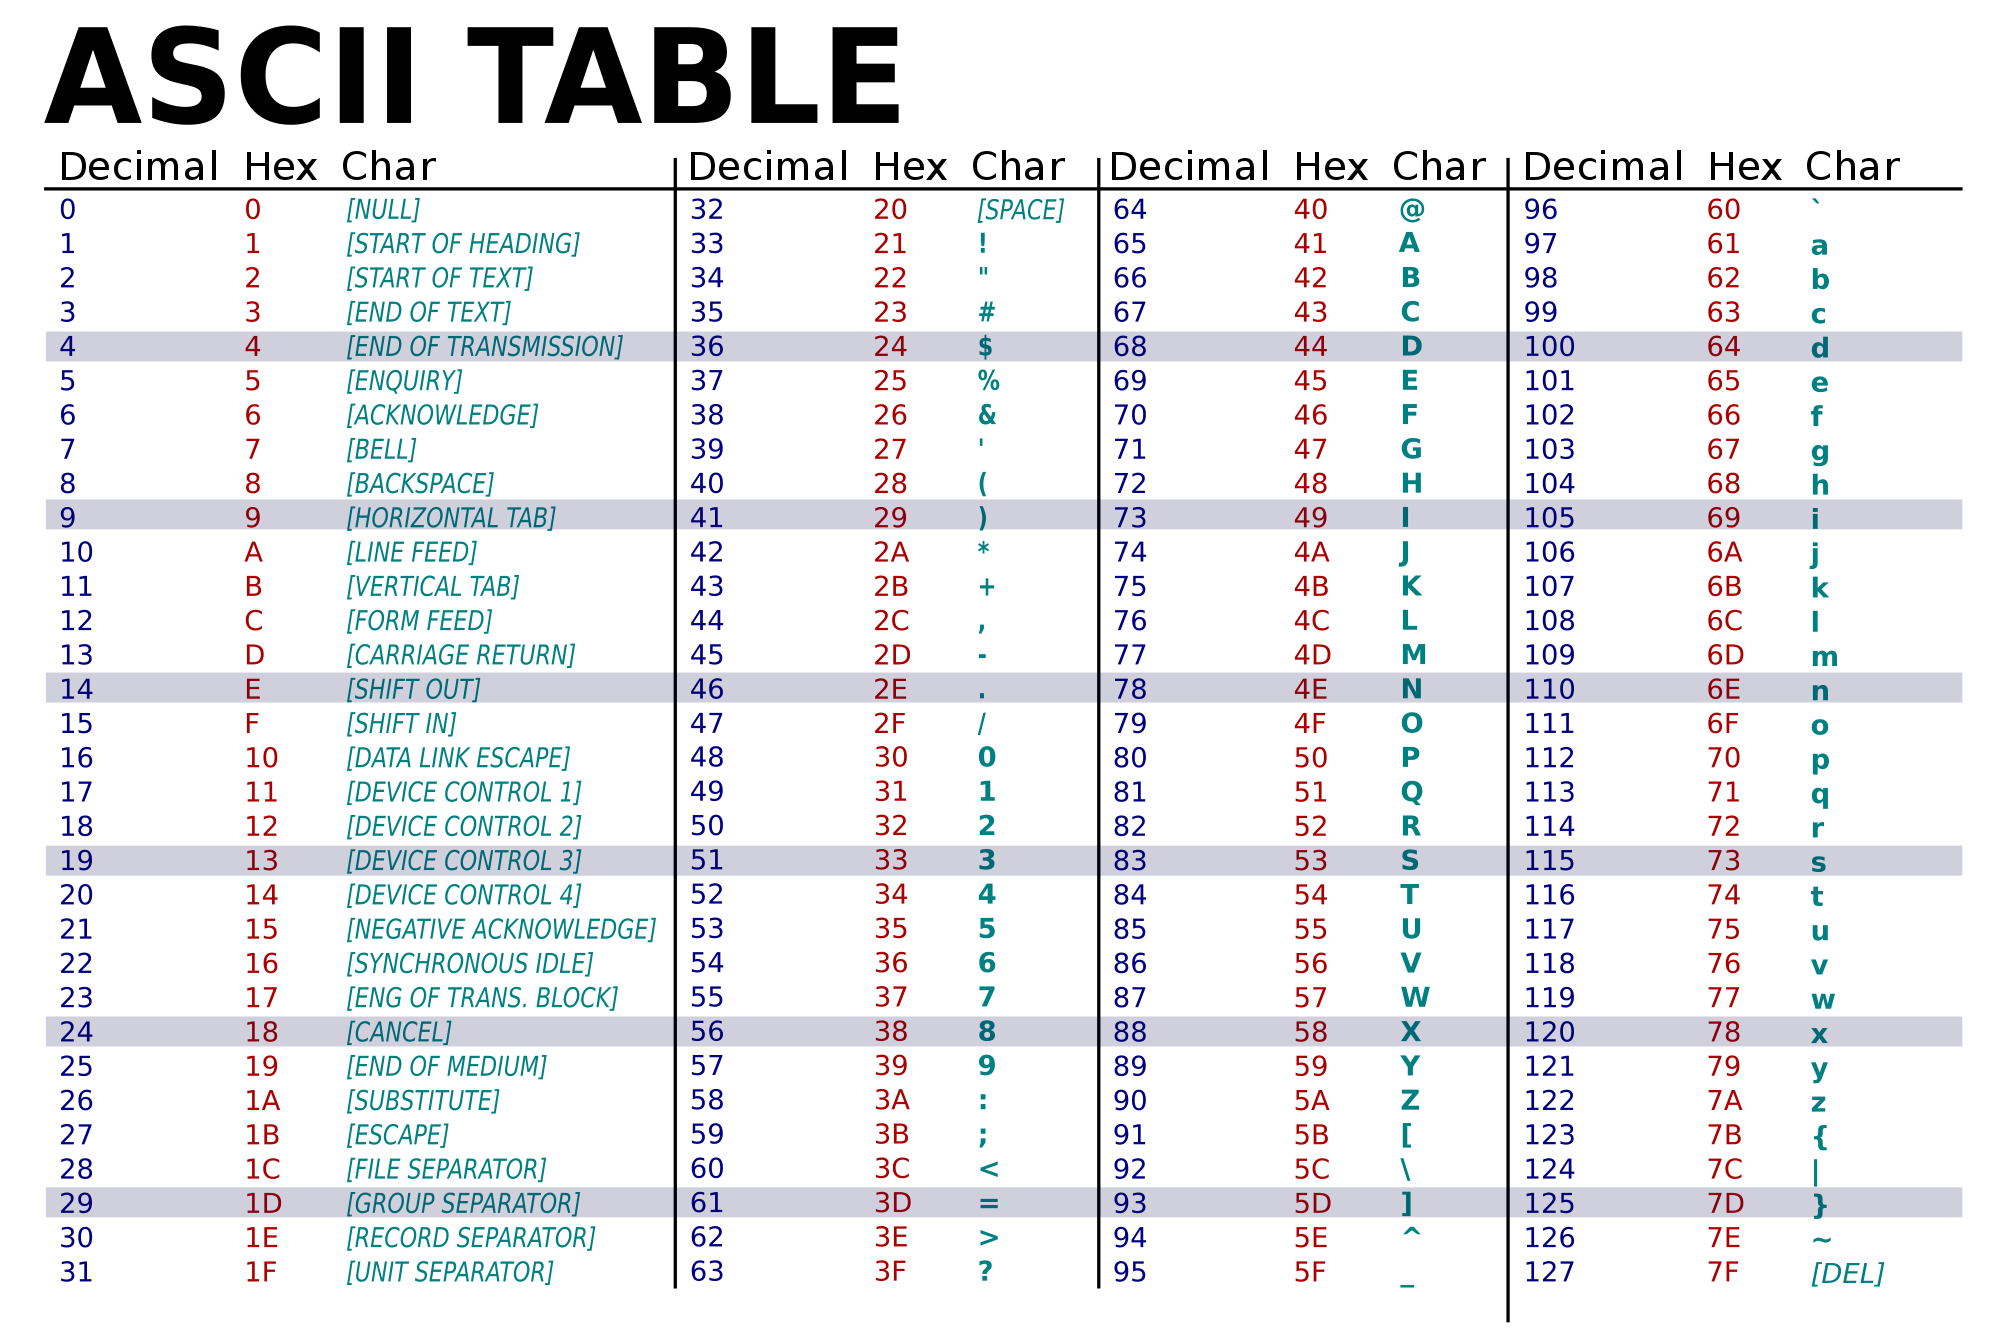
\includegraphics[scale=0.14]{images/ascii}
\end{center}
\end{frame}

\begin{frame}[fragile]
    \frametitle{Variable Naming}
    \framesubtitle{}
    
Variable Name Rules:    
\begin{itemize}
  \item<2-> May contain \mintinline{c}{a-z}, \mintinline{c}{A-Z}, 
  \mintinline{c}{0-9} or \mintinline{c}{_}
  \item<3-> May \emph{not} begin with a number
\end{itemize}

\onslide<4->{
Conventions:}
\begin{itemize}%[<+->]
  \item<5-> \mintinline{c}{under_score_casing}
  \item<6-> \mintinline{c}{UPPERCASE_UNDER_SCORE_CASING} 
  \item<7-> \mintinline{c}{camelCasingConvention}
  \item<8-> Names should be short but \emph{descriptive}
  \item<9-> Good: \mintinline{c}{initialValue}, \mintinline{c}{longitude}, \mintinline{c}{latitude}, \mintinline{c}{interestRate}
  \item<10-> Bad: \mintinline{c}{var1} \mintinline{c}{somevalue}
\end{itemize}

\end{frame}

%\subsection{Operators}

\begin{frame}[fragile]
    \frametitle{Assignment Operator}
    \framesubtitle{}

\begin{itemize}[<+->]
  \item Assignment operator: single equal sign \mintinline{c}{=}
  \item ``Place the value on the right-hand-side into the variable on the left-hand-side''
  \item Not an arithmetic equality
  \item Right hand side may be a:
  \begin{itemize}
    \item Literal: hard-coded numerical value
    \item Another variable (copy a variable's value)
    \item An arithmetic expression
  \end{itemize}
\end{itemize}  
\end{frame}

\begin{frame}[fragile]
    \frametitle{Assignment Operator}
    \framesubtitle{Examples}

\begin{minted}{c}
//declare an int variable and set it to 10:
int a;
a = 10;
//or
int a = 10;

double c = 10.5 + a * 2 - 10 / 2;
\end{minted}

\end{frame}

\begin{frame}[fragile]
    \frametitle{Arithmetic Operators}
    \framesubtitle{}

\begin{itemize}[<+->]
  \item Addition: $+ \rightarrow$ \mintinline{c}{+}
  \item Subtraction: $- \rightarrow$ \mintinline{c}{-}
  \item Multiplication: $\times \rightarrow$ \mintinline{c}{*}
  \item Division: $\div \rightarrow$ \mintinline{c}{/}
  \item Integer division: \mintinline{c}{%} gives the remainder
  \begin{itemize}
    \item \mintinline{c}{5 % 2} results in \mintinline{c}{1}
    \item \mintinline{c}{11 % 3} results in \mintinline{c}{2}
    \item \mintinline{c}{12 % 6} results in \mintinline{c}{0}
  \end{itemize} 
\end{itemize}
\end{frame}

\begin{frame}[fragile]
    \frametitle{Order of Precedence}
    \framesubtitle{}
    
\begin{itemize}[<+->]
  \item Arithmetic follows the same basic order of operations
  \item Left-to-right
  \item Multiplication/division before addition/subtraction
  \item $5 + 12 \div 2 = 11$
  \item $5 + 12 \div 2 \neq (5 + 12) / 2$
  \item Use parentheses to redefine order
  \item Best practice: use parentheses even when not necessary to indicate intent
  \item Examples:
\begin{minted}{c}
(a + 10) * (b - c)
(a * b) + (c / d)
\end{minted}
\end{itemize}

\end{frame}


\begin{frame}[fragile]
    \frametitle{Truncation}
    \framesubtitle{}
    
\begin{itemize}[<+->]
  \item Arithmetic with integers results in integers
  \item Arithmetic with \mintinline{c}{double} values results in floating-point numbers
  \item Not the same type of variables; sometimes they are \emph{incompatible}
  \item Example:
\begin{minted}{c}
//okay:
int a = 10;
double x = 10;

//in C, this results in truncation
int b = 3.14;  //b has the value 3
\end{minted}
\end{itemize}
\end{frame}


\begin{frame}[fragile]
    \frametitle{Truncation}
    \framesubtitle{}  
    
\begin{itemize}[<+->]
  \item \emph{Truncation} is when the fractional part is ``chopped off''
  \item Especially important with respect to division:
\begin{minted}{c}
int a = 10;
int b = 20;

double c = a / b;  //results in 0.0

//explicit type cast:
double d = a / (double) b; //results in 0.5
\end{minted}

\end{itemize}

\end{frame}


\section{Basic I/O}

\begin{frame}
    \frametitle{}
    \framesubtitle{}
    
    \begin{center}
    {\Huge Part III: Basic Input/Output}\\
    {\Large }
    \end{center}

\end{frame}

\begin{frame}[fragile]
    \frametitle{Basic Input/Output}
    \framesubtitle{}

\begin{itemize}[<+->]
  \item All systems support \emph{standard streams}
  \item Standard input, standard output, standard error
  \item Standard input/output library: \mintinline{c}{stdio.h}
  \item Standard input: keyboard, use \mintinline{c}{scanf}
  \item Standard output: ``console'' or terminal, use \mintinline{c}{printf}
\end{itemize}

\end{frame}

\begin{frame}[fragile]
    \frametitle{Basic Input}
    \framesubtitle{}

\begin{itemize}[<+->]
  \item \mintinline{c}{scanf}: Scan Formatted
  \item First argument: a string containing a formatting \emph{placeholder}:
  \begin{itemize}
    \item \mintinline{c}{int}: use \mintinline{c}{%d}
    \item \mintinline{c}{double}: use \mintinline{c}{%lf}
    \item \mintinline{c}{char}: use \mintinline{c}{%c}
  \end{itemize}
  \item Second argument: variable to store the value into
  \item \emph{You must place an ampersand in front of the variable}
\end{itemize}

\end{frame}

\begin{frame}[fragile]
    \frametitle{Basic Input}
    \framesubtitle{Examples}

\begin{minted}{c}
int a;
double x;

//prompt the user for an integer
printf("enter an integer: ");
scanf("%d", &a);
printf("%d\n", a);

//prompt for a double:
printf("enter a value: ");
scanf("%lf", &x);
printf("%f\n", x);
\end{minted}

\end{frame}


\begin{frame}[fragile]
    \frametitle{Basic Output}
    \framesubtitle{}

\begin{itemize}[<+->]
  \item \mintinline{c}{printf}: Print Formatted
  \item First argument: a string containing content and formatted \emph{placeholder}:
  \begin{itemize}
    \item \mintinline{c}{int}: use \mintinline{c}{%d}
    \item \mintinline{c}{double}: use \mintinline{c}{%f}
    \item \mintinline{c}{char}: use \mintinline{c}{%c}
  \end{itemize}
  \item Multiple placeholders may be used
  \item Each subsequent argument will replace each placeholder
\end{itemize}
  
\end{frame}


\begin{frame}[fragile]
    \frametitle{Basic Output}
    \framesubtitle{Examples}

\begin{minted}{c}
int a = 10;
double x = 3.14;
char initial = 'C';

printf("a = %d, x = %f and my initial is %c\n", a, x, initial);
\end{minted}

\end{frame}

\begin{frame}[fragile]
    \frametitle{Formatting Floats}
    \framesubtitle{}

\begin{itemize}[<+->]
  \item Default formatting for floating point numbers: 6 decimals of accuracy
  \item Placeholder modifier: \mintinline{c}{%n.mf} 
  \item \mintinline{c}{m}: number of decimals of accuracy
  \item \mintinline{c}{n}: \emph{minimum} number of total columns to print
  including the decimal point
  \item A negation can be used to justify left: \mintinline{c}{%-10.2f}
\end{itemize}

\end{frame}

\begin{frame}[fragile]
    \frametitle{Formatting Floats}
    \framesubtitle{Examples}
    
\begin{minted}{c}
double pi = 3.1415926;

printf("%f", pi);
printf("%.3f", pi);
printf("%.5f", pi);
printf("%10.2f", pi);
printf("%4.4f", pi);
printf("%-10.2f", pi);
\end{minted}

\end{frame}

\begin{frame}[fragile]
    \frametitle{Good Code Style}
    \framesubtitle{}

\begin{itemize}[<+->]
  \item Code must be readable and easily understood
  \item Code must be self-documenting
  \item Use accurate, descriptive variable names
  \item Consistent naming convention
  \item Good use of whitespace
  \item Consistent indentation
\end{itemize}

\end{frame}
 
\section{Exercises}

\begin{frame}
    \frametitle{}
    \framesubtitle{}
    
    \begin{center}
    {\Huge Part IV: Exercises}\\
    {\Large ~}
    \end{center}

\end{frame}


\begin{frame}
  \frametitle{Exercise}
  \framesubtitle{}

Write a program to read in three values from the user
and print their average.
  
\end{frame}


\begin{frame}
  \frametitle{Exercise}
  \framesubtitle{}

Write a program that prompts the user for the length of 
two sides of a right triangle and outputs the length of 
its hypotenuse using the Pythagorean Theorem:
%  $$h = \sqrt{a^2 + b^2}$$
%
\begin{center}
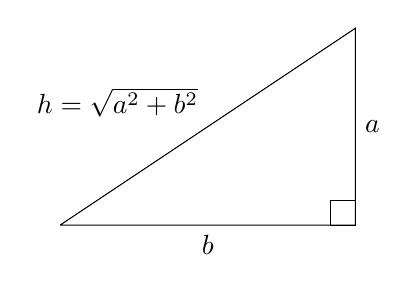
\begin{tikzpicture}[scale=1.25]%,cap=round,>=latex]

\coordinate [] (A) at (-1.5cm,-1.cm);
\coordinate [] (C) at (1.5cm,-1.0cm);
\coordinate [] (B) at (1.5cm,1.0cm);
\draw (A) -- node[above left] {$h = \sqrt{a^2 + b^2}$} (B) -- node[right] {$a$} (C) -- node[below] {$b$} (A);

\draw (1.25cm,-1.0cm) rectangle (1.5cm,-0.75cm);

\end{tikzpicture}
\end{center}


\end{frame}


\begin{frame}
  \frametitle{Exercise}
  \framesubtitle{}

Write a program to calculate mileage reimbursement.
Read in the beginning and ending odometer values as
well as a per-mile rate from the user and
display the total distance travelled as well as the
total reimbursement.  

%iterations: default printing of dollars, round
% the value

\end{frame}


\begin{frame}
  \frametitle{Exercise}
  \framesubtitle{}
  
  
Write a program to convert a number of days into
years (assume 365), weeks, and days.  For example,
if the user enters 1,000 days, it would display
``2 years, 38 weeks, 4 days.''
  
\end{frame}


\section{Command Line Input}

\begin{frame}
    \frametitle{}
    \framesubtitle{}
    
    \begin{center}
    {\Huge Part V: Noninteractive Input}\\
    {\Large Using Command Line Arguments}
    \end{center}

\end{frame}

\begin{frame}[fragile]
    \frametitle{Noninteractive Input}
    \framesubtitle{}

\begin{itemize}[<+->]
  \item Prompt/read (\mintinline{c}{printf}/\mintinline{c}{scanf}) is interactive
  \item Most real programs are \emph{not} interactive
  \item Input can be provided as Command Line Arguments (CLAs)
  \item Specified when you invoke a program: \\
  \mintinline{text}{./a.out 10 20 3.5 hello}
  \item First argument is \emph{always} the executable file name 
  \item Programs can access them using the \mintinline{c}{argv} parameter
  \item \mintinline{c}{argv[0]}, \mintinline{c}{argv[1]}, \mintinline{c}{argv[2]}, etc.
  \item Number of arguments: \mintinline{c}{argc}
  \item Each argument is a string, not a number
  \item Conversion:
  \begin{itemize}
    \item \mintinline{c}{atoi()} for \mintinline{c}{int}
    \item \mintinline{c}{atof()} for \mintinline{c}{double}
  \end{itemize}
  \item Demonstration    
\end{itemize}    

\end{frame}

\section{Toolkit: Linters}

\begin{frame}
    \frametitle{}
    \framesubtitle{}
    
    \begin{center}
    {\Huge Part VI: Toolkit Demo -- Linters}\\
    {\Large }
    \end{center}

\end{frame}

\begin{frame}[fragile]
    \frametitle{Linters}
    \framesubtitle{}


\begin{itemize}[<+->]
  \item Compilers only check for valid syntax
  \item \emph{Static analysis} tools analyze the structure of code to detect \emph{potential} bugs/errors
  \item A \emph{linter} is a utility used to identify code that may be syntactically correct but that may indicate potential bugs
  \item GCC can be used as a basic linter by forcing it to identify all warnings \\
  \mintinline{text}{gcc -Wall foo.c}
  \item Demonstration 
\end{itemize}


\end{frame}



\end{document} 
